Based on the analysis, as one of the most advanced documentation generators is Swagger UI, it will be my main inspiration.
Also, the Swagger UI is a well-known tool in the software development community, and it is used by many companies and projects.
The Swagger UI works in a way that the website is a static website by default, and the endpoints, types, and more are defined in a definition file.
This file is an OpenAPI YAML or JSON file, which is then parsed and displayed on the website~\cite{swagger-ui-definition-file}.
I think this is a good approach, as it separates the data from the view.
Thanks to this, the data can be easily changed, and the website will regenerate dynamically in the browser.
The deployment of the website is also easier, as it is just a static website, which can be hosted on any web server, and updating the definitions can be part of different deployment process.

First, I will try to analyze if I could use Swagger UI directly, or if I need to create my own website.


\section{Swagger UI for gRPC}
The first idea is to use Swagger UI and generate the OpenAPI definition file from the gRPC proto files.
This approach would have the benefit of reusing a known tool with all its features.
The issue is that OpenAPI Specification is made for HTTP APIs, which gRPC APIs, although using HTTP/2, are not~\cite{openapi-specification}.
This means that the OpenAPI Specification does not support gRPC specifics, like the streaming or mapping service methods to HTTP endpoints.
Implementation of such would require compromises on the translation layer between the two.
As described in the analysis, the grpc-gateway is an example of this translation, but it is not a perfect solution, and it has its limitations, which I want to avoid.

Another option is using Swagger UI plugin system~\cite{swagger-ui-plugins}.
This would allow me to use the swagger-ui package as a dependency and build all the gRPC specifics on top of it, including reading different specification than OpenAPI\@.
The positive side of this approach is that I would be able to use the Swagger UI design.
But, on the other hand, I would need to reimplement almost every single part in order to be able to work with gRPC specifics, and in the future maintain compatibility with possible Swagger UI updates.
This would leave me only with a page skeleton, which is a toolbar and a background color.
I do not see that as a significant advantage over creating my own website.

In the end, I have decided to create my own website, which will be inspired by the Swagger UI design, but it will be adjusted to the gRPC specifics.


\section{gRPC-Web Limitations}
% gRPC-Web limitations, and how it affects the design
% Possibility of full gRPC server implementation in the future, but also may-be not necessary if gRPC-Web supports it
% grpc-web-text and grpc-application content types
Previously I have mentioned the gRPC-Web limitations.
The most important for my design is a lack of support for client streaming and bidirectional streaming, but its implementation is on the roadmap.
This means that the website will not be able to execute these types of methods, and the execution will be limited to unary and server streaming methods only.
It does not affect the design of the website, though, the website can still show all relevant documentation and have the implementation ready when gRPC-Web developers add support.

If gRPC-Web support for client streaming and bidirectional streaming will not be added any time soon, I will prepare a way to use custom gRPC server proxy implementation.
If that implementation was provided, the website will be able to use it, and the user will be able to use all gRPC methods, including client streaming and bidirectional streaming.
This solution will not be part of my thesis, but I will prepare the website for it, so it can be added (or removed altogether) in the future.


The server streaming also has a limitation in gRPC-Web, which is that it works only in \textit{application/grpc-web-text} format~\cite{grpc-web}.
This means that the payload is base64 encoded, and it is not possible to use the \textit{application/grpc-web+proto} content type, which uses payload in binary format.
Only unary calls support both \textit{an application/grpc-web+proto} and \textit{application/grpc-web-text} content types.
Therefore, unary requests will feature a content type selection, where user will be able to change it.


\section{gRPC Reflection Possibility}
% Discuss the options and possibilitions
Before I start designing the website architecture, I need to decide how the gRPC reflection as a data source could be used compared to the proto files.
Any tool using gRPC reflection has to support connection using gRPC itself.
Therefore, it is not possible to use it directly in the browser.
There will need to be a server-side tool or client, which will connect to the gRPC server and get the reflection data.
The gRPCurl tool mentioned in the analysis allows not only creating the client, but also to export a \enquote{protoset}file.
This is a file containing the reflection metadata in its own format.
This file can be then used instead of direct gRPC server as a reflection source.
But it can also be read by different tools than grpcul.
For example, the gRPC UI tool elevates this in its own implementation~\cite{grpc-grpcui}.
This will allow for the documentation website to either use the protoset file directly, or convert the protoset file to a different common format, which will be then used by the website.

% Issue with comments in Reflection, reflection feasability
The limitation of the gRPC reflection is that it does not provide comments from the proto files.
This means that the website will not be able to show the comments, which are part of the proto files, if the reflection is used.
This is a significant limitation, as the comments are part of the documentation, and they are important for the user to understand the methods and types.
The good thing is that it is being tracked on GitHub (\url{https://github.com/grpc/grpc/issues/22680}) by the gRPC developers, and when it is implemented, the documentation website will be able to use it.
For now, if documentation comments are required, the proto files will have to be used as the data source.


\section{Architecture}
The architecture of the website will be based on the Swagger UI, but it will be adjusted to the gRPC specifics.
The website will be a static website, which will take a gRPC definition file for showing all gRPC related parts.
The gRPC definition file from the proto files or gRPC reflection and its format will be most probably either JSON or YAML\@.
These formats are common in software development, and they are also used by the Swagger UI, which I take the inspiration from.

I have created a diagram of the website architecture, which is shown in the figure~\ref{fig:grpcflair-architecture}.
There are two places where the generation of the common format starts.
The first one is from the .proto, the second one is from the gRPC reflection.
Both methods will generate the same format, which will be then used by the website.
The website will be a static website, which will be generated from the common format on the fly using JavaScript.
The user of the website will be able to see all the methods, types, and enums, which are defined in the gRPC definition file.
They will also be able to call the methods and see the responses on the website.
When they invoke the request, the website will select the correct backend (gRPC-Web or other implementation) and it will the server.
The server then returns the response, which is then displayed on the website (the responses can be shown gradually as for example the server streams responses).

% The overall process description - state diagram - (with the help of the diagram I have)
% Swagger UI JSON inspiration

\begin{figure}[hbt!]
    \centering
    \captionsetup{justification=centering}
    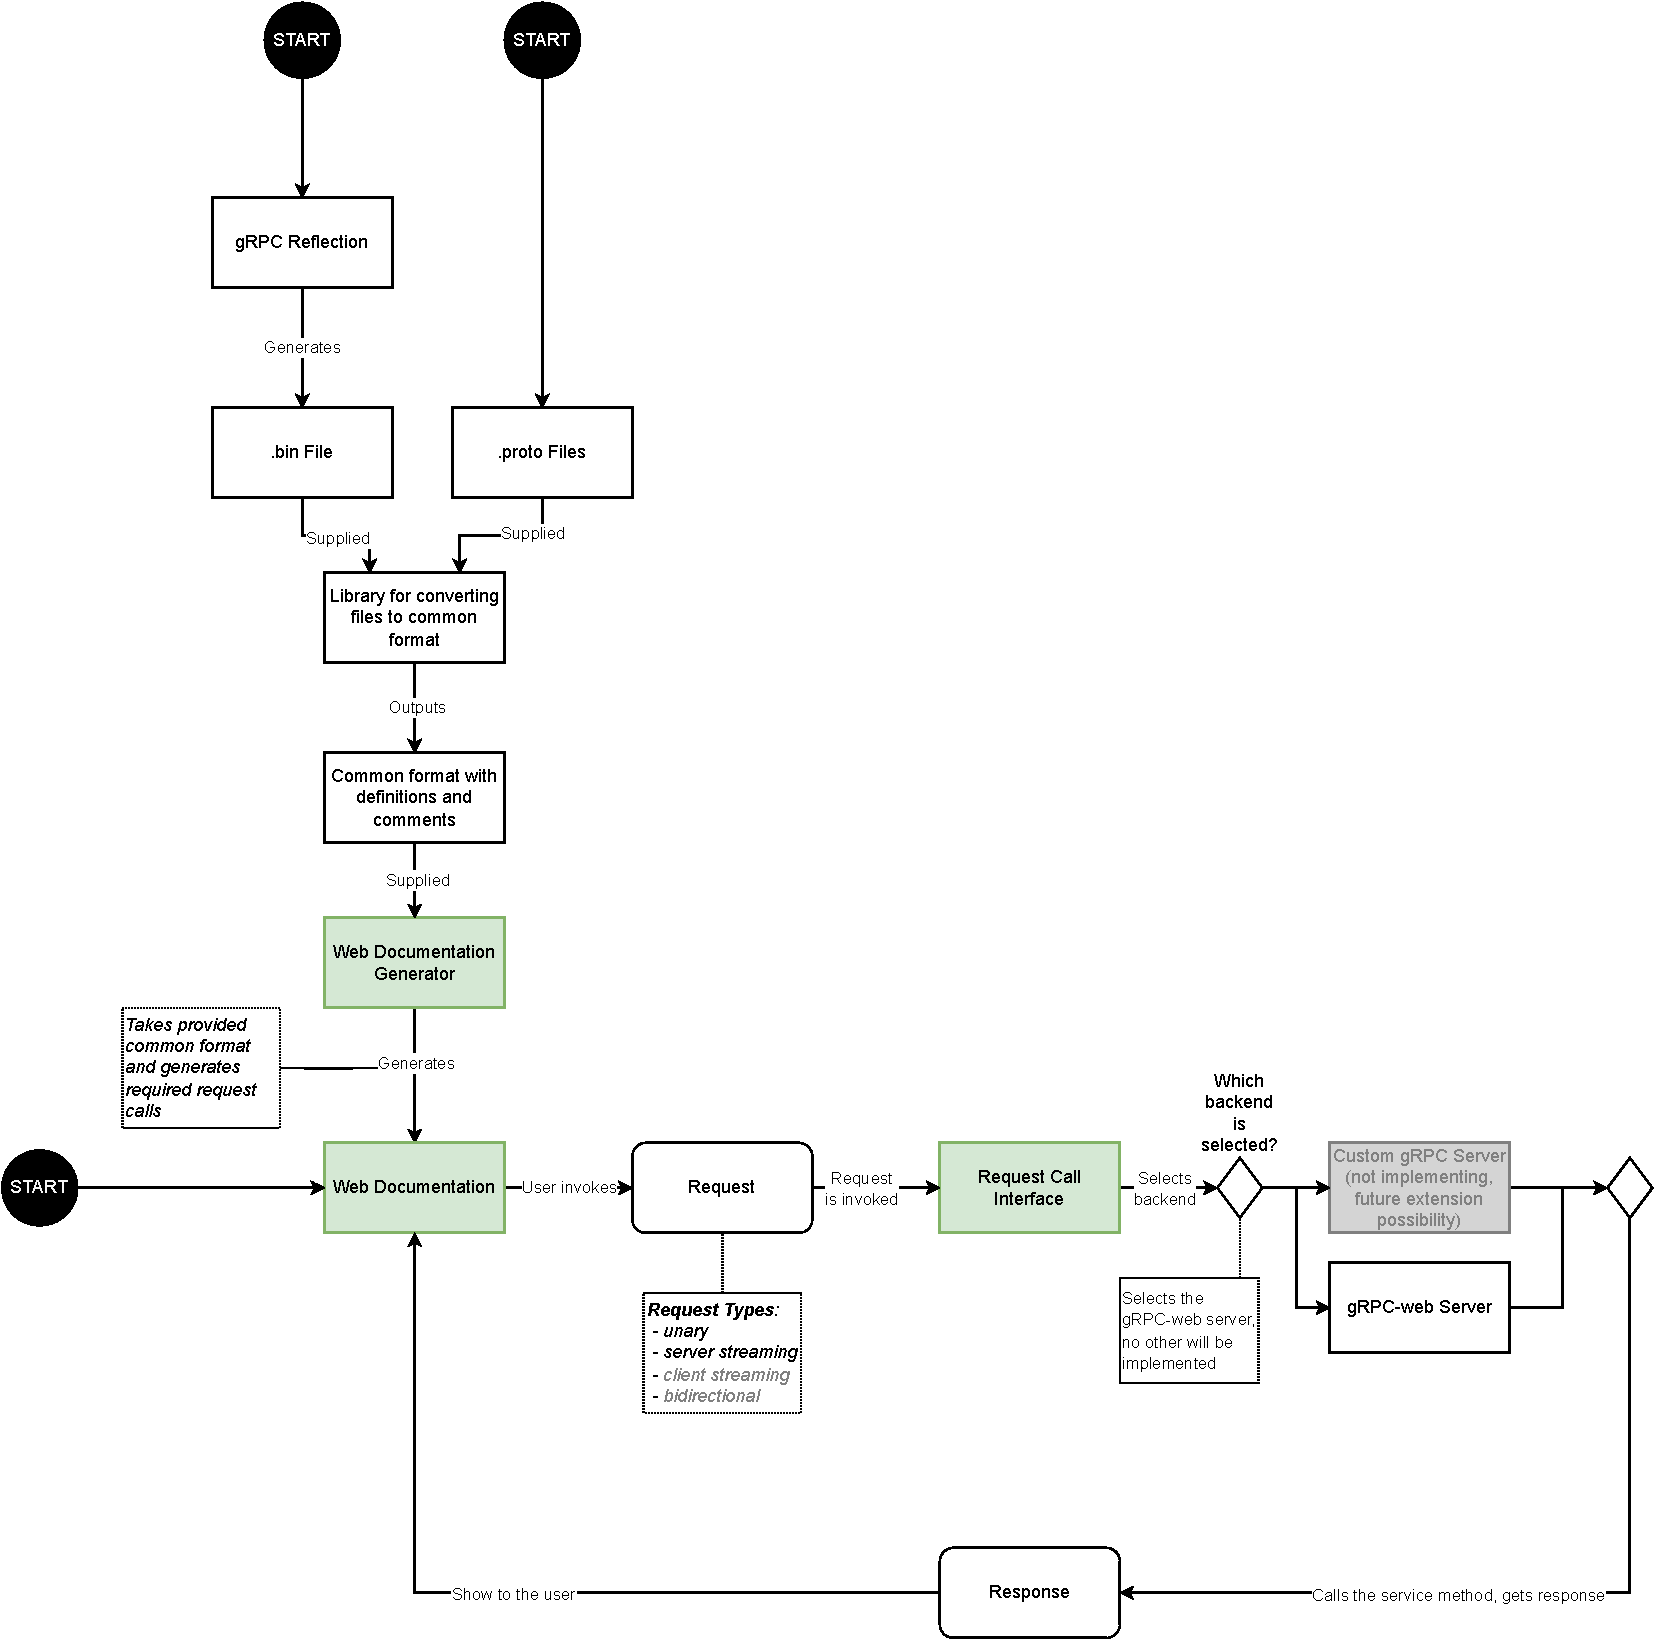
\includegraphics[width=1.0\textwidth]{images/design/grpcdoc-architecture}
    \caption{Architecture}
    \label{fig:grpcflair-architecture}
\end{figure}


\section{Common Format}

% TODO: Probably not even consider, because already discussed earlier
%\subsection{OpenAPI}
% Why not use OpenAPI -> It's made for REST, not gRPC, I would have to map it -> already existing solutions

\subsection{grpc-protoc-gen-doc}

\subsection{gnostic}

\subsection{proto3-json-serializer}

\subsection{protobufjs}
% Protobufjs, protobufjs-cli

\subsection{Summary}
% Why not use my own parsing


\section{Website Design}

\subsection{Proto Files Generator}

\subsection{gRPC Reflection Generator}
% Discuss the options and possibilitions

\subsection{Website Wireframe}
% Inspiration and main focus
% Section: Main Page
\ref{fig:wireframe-main-layout}

\begin{figure}[hbt!]
    \centering
    \captionsetup{justification=centering}
    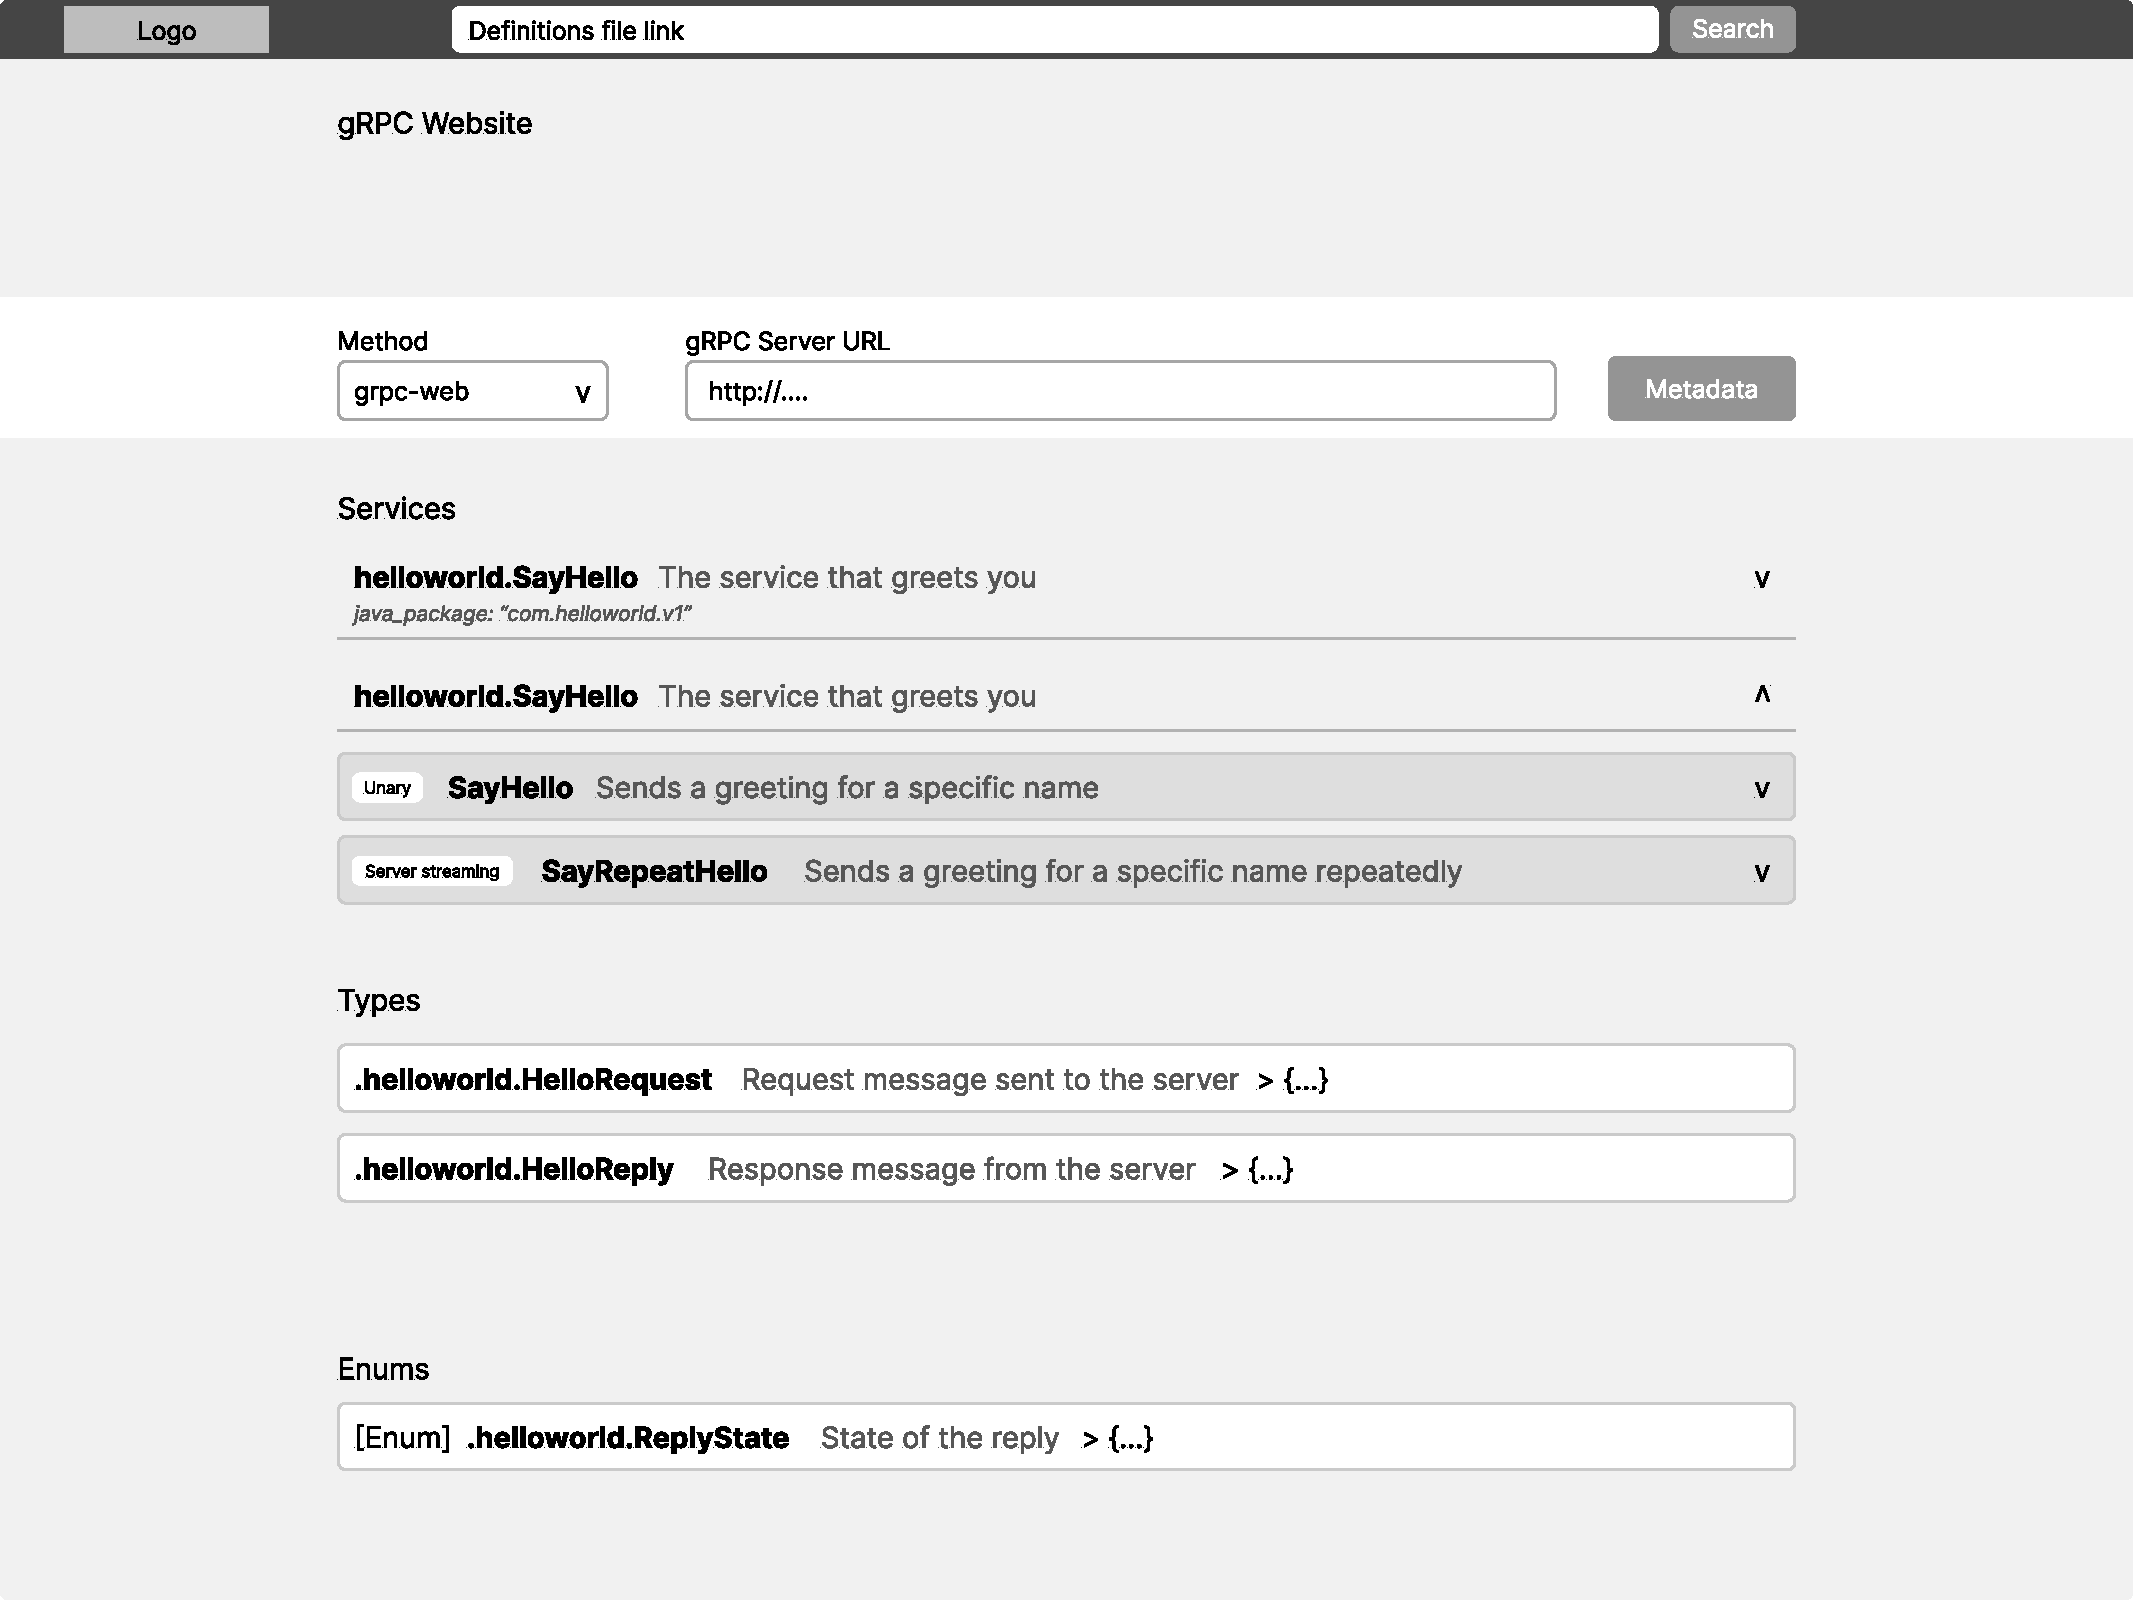
\includegraphics[width=1.0\textwidth]{images/design/wireframes/main-layout}
    \caption{Main Layout Wireframe}
    \label{fig:wireframe-main-layout}
\end{figure}

\subsubsection{Method Wireframe}
% Section: Method, and it's detail with forms, JSON, etc
\ref{fig:wireframe-method}

\begin{figure}[hbt!]
    \centering
    \captionsetup{justification=centering}
    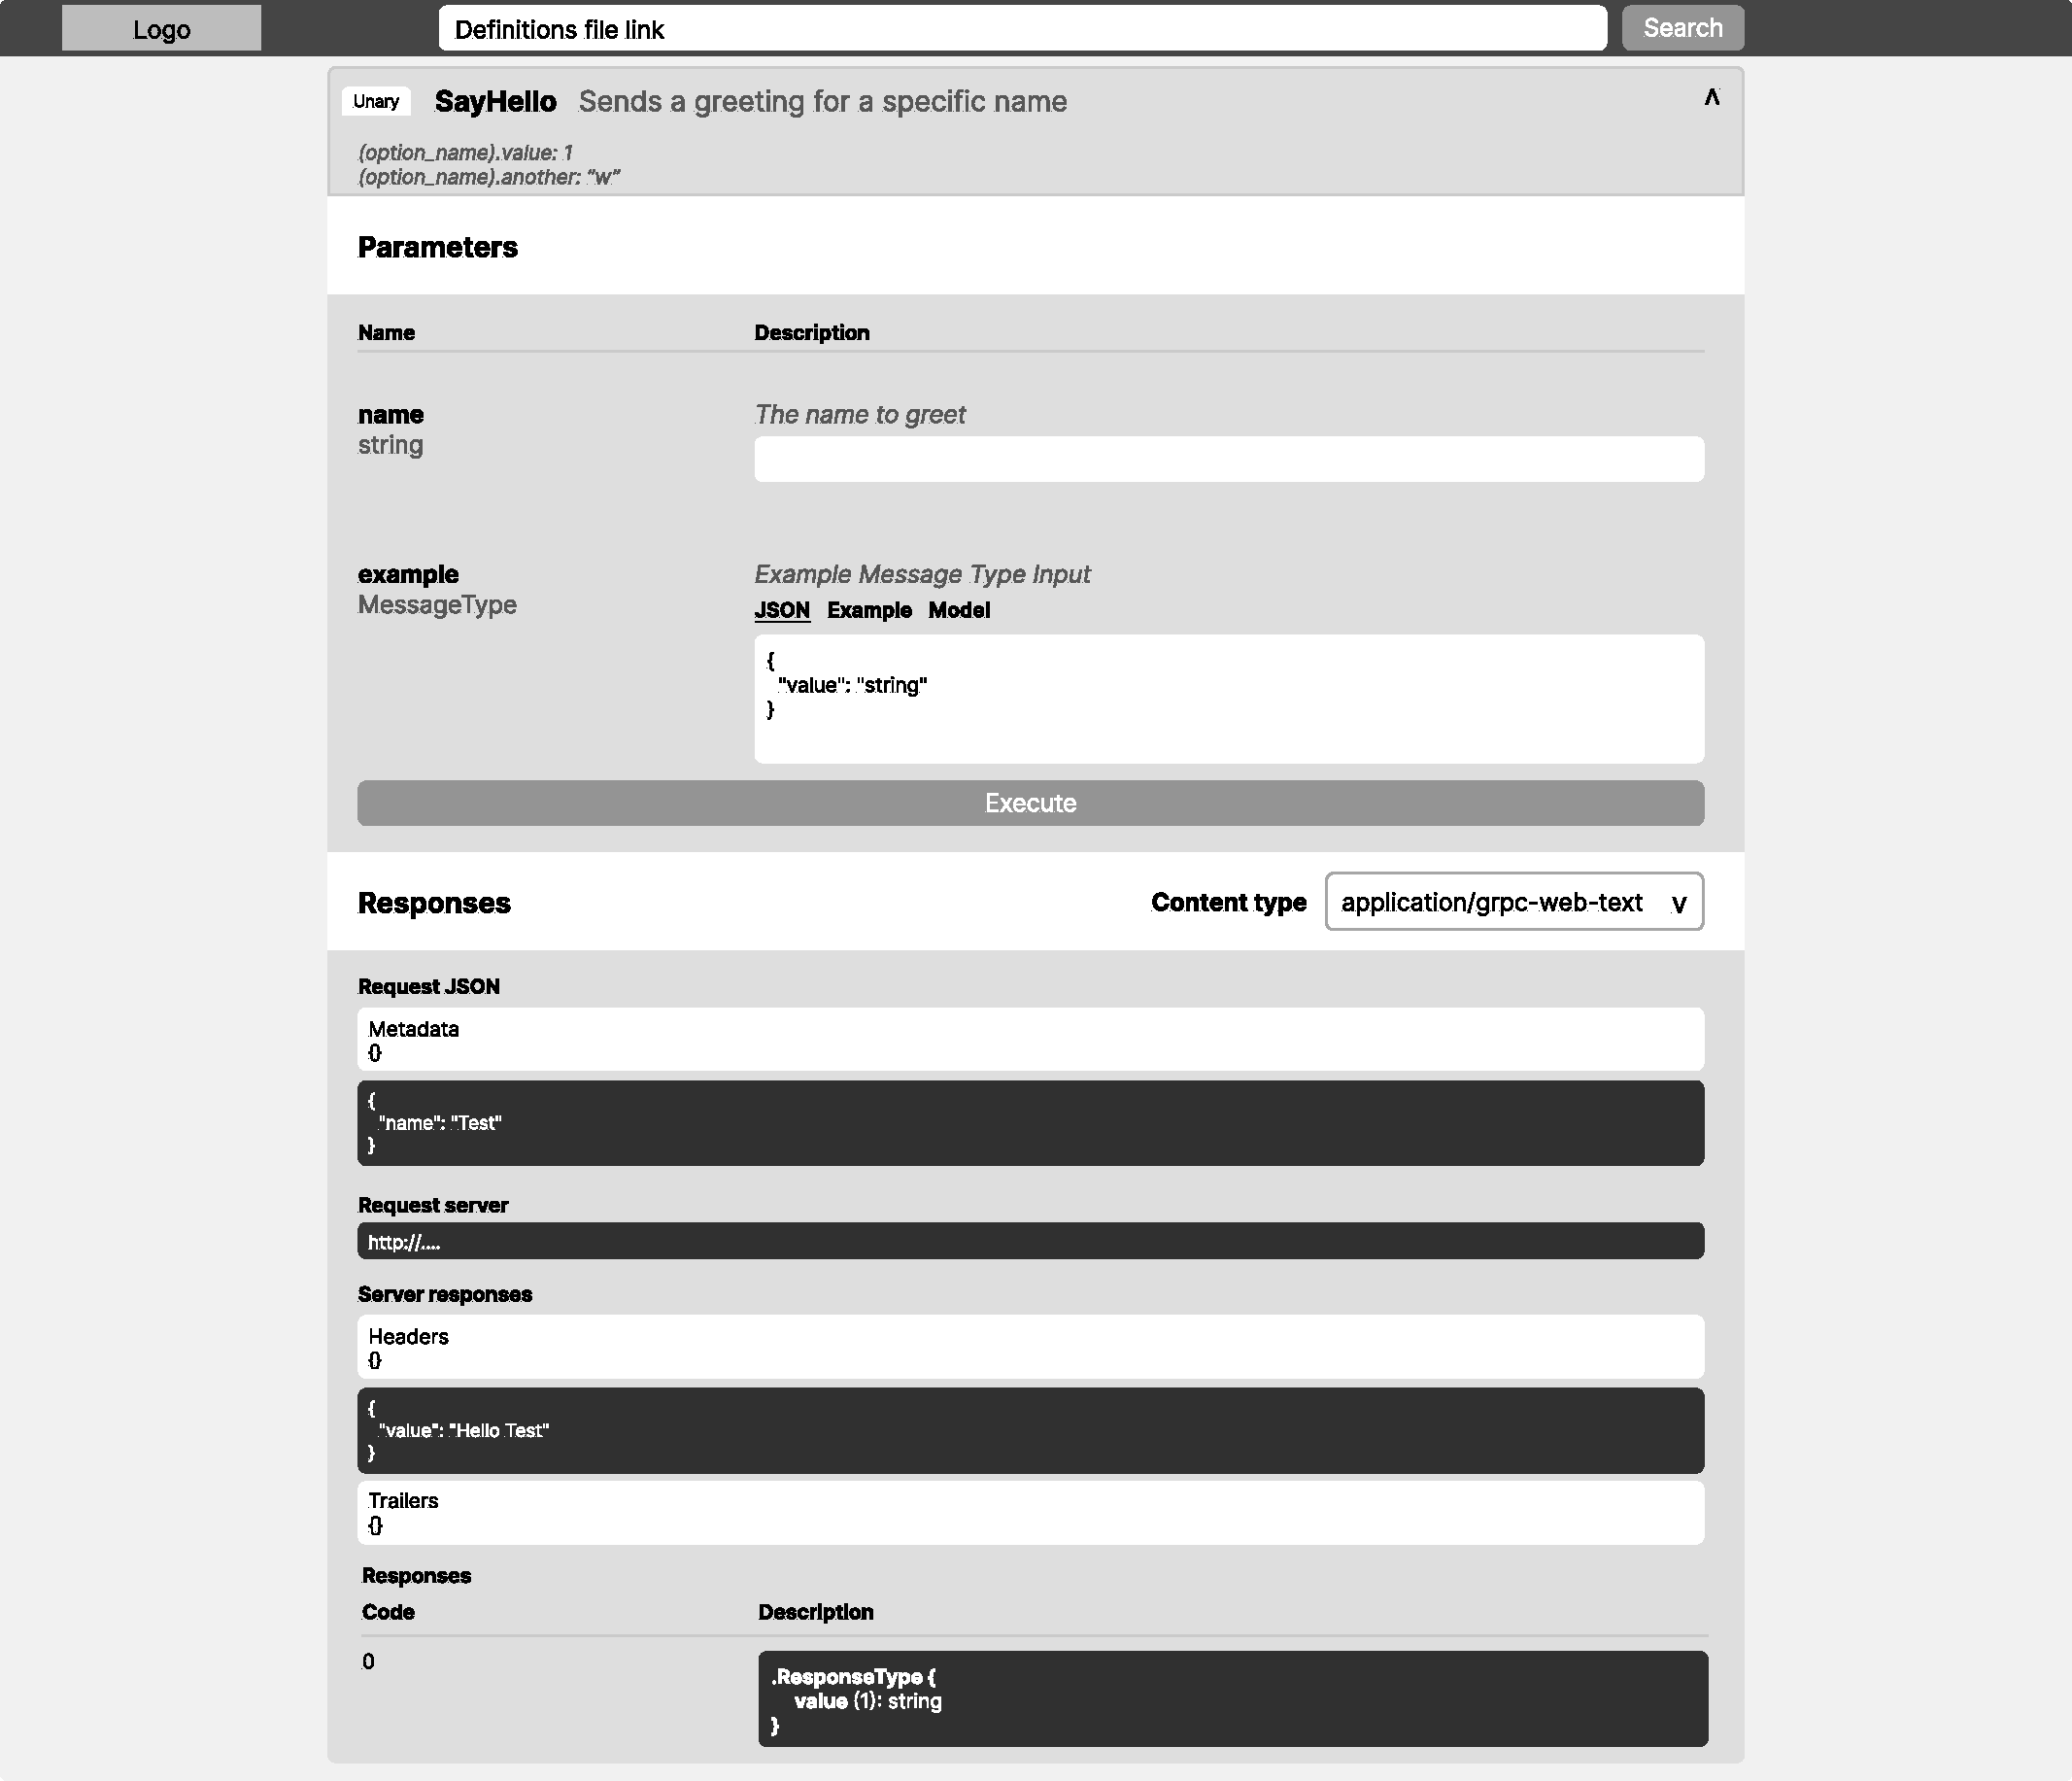
\includegraphics[width=1.0\textwidth]{images/design/wireframes/method}
    \caption{Method Wireframe}
    \label{fig:wireframe-method}
\end{figure}

\subsubsection{Type and Enum Wireframe}
% Section: Type & Enum
\ref{fig:wireframe-type}
\ref{fig:wireframe-enum}

\begin{figure}[hbt!]
    \centering
    \captionsetup{justification=centering}
    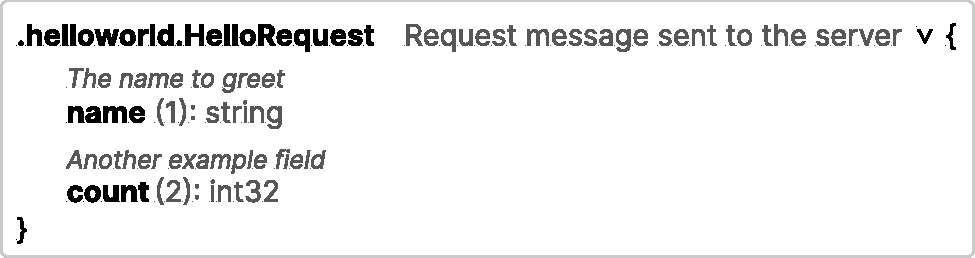
\includegraphics[width=0.8\textwidth]{images/design/wireframes/type}
    \caption{Type Wireframe}
    \label{fig:wireframe-type}
\end{figure}

\begin{figure}[hbt!]
    \centering
    \captionsetup{justification=centering}
    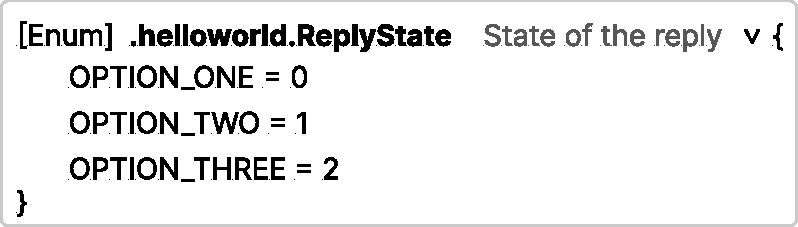
\includegraphics[width=0.8\textwidth]{images/design/wireframes/enum}
    \caption{Enum Wireframe}
    \label{fig:wireframe-enum}
\end{figure}


\section{Fulfillment of Requirements}
%Samotné grafické rozhraní aplikace splňuje požadavek N1.
%Zobrazení dialogového okna s informacemi pro inicializaci obrazu softwaru Syllabus Plus splňuje požadavek F1.
%Uspořádání dat do sloupců a rozdělení obrazovky na dvě části splňuje požadavek F16.
%Libovolný výběr dat a částečné převody u všech pohledů splňuje požadavky F2, F3, F5, F6, F9, F10 a částečný export u pohledu časových lístků splňuje požadavky F17 a F18.
%Požadavek F4 je splněn pouhým přidáním sloupce navíc k pohledu místností, není nutné cokoli v návrhu měnit, jedná se pouze o implementaci.
%Požadavek F7 je implementačně závislý, nesouvisí s návrhem rozhraní.
%Možnost výběru informací u převodu časových lístků pokrývá požadavek F8.
%Tlačítko pro spárovaní položek splňuje požadavek F11.
%Dialogové okno před převodem dat do systému Syllabus Plus splňuje požadavek F12 a dialogové okno při exportu dat splňuje požadavek F13.
%Rozdíly mezi položkami zobrazené pomocí barevné tečky splňují požadavek F14.
%Dialogové okno zobrazené po kliknutí na časový lístek splňuje požadavek F15.
%Výběr semestru v levém horním rohu splňuje požadavek F19.
%Filtr u každého sloupce splňuje požadavek N2.
%
%Tímto uživatelské rozhraní splňuje všechny požadavky.

